\documentclass[twoside,11pt]{article}

% Supplementary Material (online appendix) for main.tex.
% Build order: main.tex, then supplement.tex, then main.tex again (xr-hyper).
\PassOptionsToPackage{hypertexnames=false}{hyperref}
\usepackage{xr-hyper}
\usepackage[abbrvbib]{jmlr2e}
% jmlr2e's proof environment takes no optional argument; allow one.
\renewenvironment{proof}[1][Proof]{\par\noindent{\bfseries #1\ }\ignorespaces}{\leavevmode\unskip\penalty9999\hbox{}\nobreak\hfill\quad\hbox{\BlackBox}\par\vspace{2mm}}

\usepackage{amsmath}
\usepackage{mathtools}
\usepackage{bm}
\usepackage{booktabs}
\usepackage{array}
\usepackage{microtype}
\usepackage{needspace}
\usepackage{xcolor}
\usepackage{algorithm}
\usepackage[noend]{algpseudocode}
\usepackage{enumitem}
\usepackage{placeins}
% lastpage is not loaded here: its LastPage label would collide with
% main.tex through xr-hyper.
\usepackage[capitalise,nameinlink]{cleveref}
\setlist{itemsep=2pt,topsep=4pt}

% ---------- Notation ----------
\newcommand{\R}{\mathbb{R}}
\newcommand{\E}{\mathbb{E}}
\newcommand{\Prob}{\mathbb{P}}
\DeclareMathOperator{\Var}{Var}
\DeclareMathOperator{\rank}{rank}
\DeclarePairedDelimiter{\abs}{\lvert}{\rvert}
\DeclarePairedDelimiter{\norm}{\lVert}{\rVert}
% \SND denotes the population diversity mu(D) of any dissimilarity table;
% the MARL instance is written \mathrm{SND} explicitly.
\newcommand{\SND}{\mu}
\newcommand{\SNDG}{\widehat{\mu}_{G}}
\newcommand{\Pairs}{\mathcal{P}}
\newcommand{\sigmamain}{\sigma^2_{\mathrm{main}}}
\newcommand{\sigmaint}{\sigma^2_{\mathrm{int}}}
\newcommand{\sigmatot}{\sigma^2_{\mathrm{tot}}}
\newcommand{\SNDdes}{\mu_{\mathrm{des}}}
\newcommand{\muhat}{\widehat{\mu}}
\newcommand{\Dmat}{\mathbf{D}}
\newcommand{\Rmat}{\mathbf{R}}
\newcommand{\one}{\mathbf{1}}
\newcommand{\Sym}{\mathfrak{S}}

\jmlrheading{XX}{2026}{S1--\pageref{supp:last}}{11/26}{--}{XX-XXXX}{Shawn Ray}
\ShortHeadings{Supplementary Material}{Ray}
\firstpageno{1}

\raggedbottom
\brokenpenalty=10000
\emergencystretch=1.5em
\hyphenation{Cob-bold Theorem Theorems Proposition Propositions Corollary Corollaries Section Sections Appendix Appendices PyTorch NumPy Dieng Bettini November}
\externaldocument{main}
\renewcommand{\thesection}{S\arabic{section}}
\renewcommand{\thetable}{S\arabic{table}}
\renewcommand{\thefigure}{S\arabic{figure}}
\renewcommand{\theequation}{S\arabic{equation}}
\renewcommand{\thepage}{S\arabic{page}}
\renewcommand{\thetheorem}{S\arabic{theorem}}
\begin{document}

\title{Supplementary Material for\\ ``Measuring Pairwise Diversity\\ with Linearly Many Comparisons''}

\author{\name Shawn Ray \email shawnray@cmu.edu \\
       \addr Carnegie Mellon University\\
       5000 Forbes Avenue\\
       Pittsburgh, PA 15213, USA}

\editor{}

\maketitle

\noindent This supplement contains a table of notation
(\Cref{app:notation}), details of every experiment (\Cref{app:exp-details}),
additional results (\Cref{app:additional}), exact formulas for separable
dissimilarities (\Cref{app:separable}), and the proofs of
\Cref{prop:lower,prop:sparse-anatomy,prop:dico} together with five remarks on
the theory (\Cref{app:supp-proofs}). Theorems, sections, figures, and equations without the
prefix~S refer to the main article.

% Notation table (moved from the main appendix to the supplement).
\section{Notation}
\label{app:notation}

\begin{table}[h]
\centering
\small
\caption{\textbf{Notation.} Symbols used in the main article and in this supplement.}
\label{tab:notation}
\vspace{4pt}
\begin{tabular}{@{}ll@{}}
\toprule
Symbol & Meaning \\
\midrule
$n$, $[n]$ & population size and index set $\{1,\dots,n\}$ \\
$\Pairs$, $N$ & unordered pairs of individuals and their number $\binom{n}{2}$ \\
$D=(d_{ij})$ & dissimilarity table (symmetric, non-negative, zero diagonal) \\
$\mu=\SND(D)$ & pairwise diversity, the mean of $d_{ij}$ over $\Pairs$ (SND in MARL) \\
$S_i$ & row sum $\sum_{j\ne i}d_{ij}$ \\
$a_i$ & distinctiveness of individual $i$, $(S_i-(n-1)\mu)/(n-2)$ \\
$r_{ij}$, $R$ & relational residual $d_{ij}-\mu-a_i-a_j$ and its matrix \\
$\sigmatot,\sigmamain,\sigmaint$ & total, distinctiveness, and relational energies (\Cref{def:anatomy}) \\
$\kappa$ & ratio $\sigmamain/\sigmaint$; efficiency gain $\approx1+\kappa$ (\Cref{cor:efficiency}) \\
$G=([n],E,w)$ & comparison design with total weight $W$ \\
$\delta_i$, $\bar\delta$ & weighted degree of $i$ in $G$ and its average $2W/n$ \\
$\SNDG$ & design estimate \eqref{eq:design-estimator} of $\mu$ \\
$k$, $m$ & degree of a regular design and its number of comparisons $nk/2$ \\
$H$, $\sigma$ & base graph and uniform random relabeling of a design, $G=\sigma(H)$ \\
$T$, $T_U$ & balanced (randomized regular) and uniform-pair estimates of $\mu$ \\
$v_{n,k}$ & metric-universal bound on $\Var(T)/\mu^2$ (\Cref{thm:metric}) \\
$\lambda_2,\lambda_n$ & second largest and smallest adjacency eigenvalues of $G$ \\
$\norm{\cdot}_*$ & nuclear norm \\
$\SNDdes$, $e$ & diversity target and relative estimation error in control \\
\bottomrule
\end{tabular}
\end{table}


% ============================================================
% app_exp_details.tex -- experimental details
% ============================================================
\section{Experimental Details}
\label{app:exp-details}

All code, tables, and logs are released with the paper. Unless stated
otherwise, estimators are compared at a matched budget of $m=nk/2$ evaluated
pairs, with $k\in\{1,2,4,8,16\}$ and $k<n-1$ ($k\le8$ in the law checks of \Cref{sec:exp-laws}).

\subsection{Synthetic populations}
\label{app:exp-details:synthetic}

Each synthetic population is a set of $n$ behavior embeddings $x_i$, and the
dissimilarity is the Euclidean distance $d_{ij}=\norm{x_i-x_j}_2$, so every
table is a pseudometric table. $Z$ denotes a matrix of independent standard
normal entries, $g_i$ a vector of independent standard normal entries, and $e_1$ the first basis vector. Table~\ref{tab:synthetic}
lists the generators. Each family is drawn at $n\in\{50,100,200\}$ with two seeds for the exact-law checks and three further times at $n=200$ for the matched-budget comparison.

\begin{table}[ht]
\centering
\small
\caption{\textbf{Synthetic families.} Labels are ordered by role (by angle for the
continuum), so fixed, unshuffled designs meet the structure in its least
favorable orientation.}
\label{tab:synthetic}
\begin{tabular}{@{}>{\raggedright\arraybackslash}p{2.4cm}>{\raggedright\arraybackslash}p{6.9cm}>{\raggedright\arraybackslash}p{4.9cm}@{}}
\toprule
Family & Generator & What it models \\
\midrule
near-simplex & $X=I_n+0.05\,Z_{n\times n}$ (rows $x_i$) & equidistant team with idiosyncratic noise \\
heterogeneous scale & $x_i=\omega_i z_i$, $\log \omega_i\sim\mathcal N(0,0.6^2)$, $z_i\sim\mathcal N(0,I_{64})$ & members differ in idiosyncrasy \\
one outlier & near-simplex, then $x_1\leftarrow 6\,x_1$ & one specialist or faulty member \\
two roles & $x_i=3e_1\,\one\{i>n/2\}+0.3\,g_i$, $g_i\sim\mathcal N(0,I_8)$ & two equal roles \\
unequal roles & four roles of sizes $40/30/20/10\%$, centers $3\,Z_{4\times 8}$, noise $0.3$ & unbalanced role structure \\
continuum & $x_i=(\cos\theta_i,\sin\theta_i)+0.02\,g_i$, $\theta_i=2\pi i/n$ & a continuum of behaviors \\
\bottomrule
\end{tabular}
\end{table}

\subsection{Designs compared}
\label{app:exp-details:designs}

Table~\ref{tab:design-list} lists all estimators; ``Balanced'' in \Cref{tab:e2} and \Cref{fig:designs} is the round-robin design. Randomized estimators are
replicated $3{,}000$ times for the exact-law validation and $2{,}000$ times for
the matched-budget comparison. Landmarks use $\max\{1,\operatorname{round}(m/(n-1))\}$
random pivots and evaluate all pairs touching them, about $m$ pairs (at $k=1$ a single pivot already costs $n-1\approx2m$ pairs). Symmetrized nearest-neighbor graphs, built from the dissimilarity table
itself, have between $m$ and $2m$ edges; using the true table is the best case for a local graph and the worst case for estimating $\mu$, because it selects the smallest dissimilarities. Where a baseline uses more pairs than the budget, the comparison favors that baseline. The fixed expander is a union of $k$ random perfect matchings; each draw is held fixed, so its error is pure bias, and we report the root-mean-square error over $100$ independent draws. For $k=1$ such a union is a perfect matching and for $k=2$ a union of cycles, so neither is an expander; this affects only the smallest budgets. Repeated edges are possible at every $k\ge2$ and are kept with multiplicity, so the graph is a $k$-regular multigraph rather than a simple graph as in \Cref{thm:balanced}; averaged over draws, its mean squared error is that of the balanced design times $(n-2)/(n-1-k)$, which is below $1.09$ for $n=200$ and $k\le16$. The check of \Cref{thm:fixed-spectral} uses simple random
$k$-regular graphs ($20$ per $k$) and the ring lattice.

\begin{table}[ht]
\centering
\small
\caption{\textbf{Estimators of the mean pairwise dissimilarity.} The first two are the
balanced designs of Theorem~\ref{thm:balanced}. The last three are fixed graphs (the expander is drawn at random, then held fixed).}
\label{tab:design-list}
\begin{tabular}{@{}>{\raggedright\arraybackslash}p{3.2cm}>{\raggedright\arraybackslash}p{7.6cm}>{\raggedright\arraybackslash}p{3.4cm}@{}}
\toprule
Design & Pairs evaluated & Weights \\
\midrule
round-robin & $k$ random rounds of the circle-method \mbox{1-factorization}, relabeled & uniform \\
permuted circulant & $i\sim i\pm1,\dots,\pm\lfloor k/2\rfloor$ on a random cyclic order, plus $i\sim i+n/2$ if $k$ is odd & uniform \\
uniform pairs & $m$ pairs without replacement & uniform \\
Bernoulli (HT) & each pair with probability $p=m/N$ & $1/p$, normalized by $N$ \\
Bernoulli (ratio) & each pair with probability $p=m/N$ & uniform over realized pairs \\
agent subsampling & all pairs among $s$ random agents, $\binom s2\approx m$ & uniform \\
landmarks & all pairs touching $\approx m/(n-1)$ random reference agents (at least one) & uniform \\
nearest neighbors (fixed) & each agent's $k$ most similar agents (local graph) & uniform \\
fixed ring & the same circulant graph in the given labeling & uniform \\
random expander (fixed) & union of $k$ random perfect matchings, each held fixed; RMSE over $100$ independent draws & uniform \\
\bottomrule
\end{tabular}
\end{table}

\subsection{Trained multi-agent teams in VMAS}
\label{app:exp-details:vmas}

We train heterogeneous teams with independent PPO on VMAS \citep{bettini2022vmas}.
Each agent has its own $2\times64$ tanh multilayer perceptron (MLP) policy with a state-independent
log standard deviation, and there is no parameter sharing. Each PPO iteration
collects $64$ steps in each of $128$ parallel environments, which is $8{,}192$
environment steps, with episodes capped at $200$ steps.
Runs were launched in three waves with wall-clock budgets of $13$, $23$, and
$14$ minutes, respectively, on shared GPUs, so the iterations reached vary
(Table~\ref{tab:vmas-runs}); teams are observed during training and are not
claimed to be converged. Table~\ref{tab:ippo-hparams} lists the remaining
hyperparameters.

Behavioral distances follow SND \citep{bettini2025snd}. At each saved iteration,
all $n$ policies are evaluated on a shared pool $\mathcal B$ of $4{,}096$ observations sampled
from that \mbox{iteration's} rollout, with all agents' observations pooled. For diagonal
Gaussian policies,
\[d_{ij}=\frac{1}{|\mathcal B|}\sum_{o\in\mathcal B}\big(\norm{m_i(o)-m_j(o)}_2^2+\norm{\sigma_i(o)-\sigma_j(o)}_2^2\big)^{1/2},\]
where $m_i(o)$ and $\sigma_i(o)$ are agent $i$'s action mean and standard deviation; that is, the $W_2$ distance between the two agents' Gaussian action distributions at $o$, averaged over $\mathcal B$. Tables are saved on a wave-specific schedule
of early iterations and always at the final iteration. Two semi-synthetic variants
are built from each final team: one with agent~$1$'s weights reset to their initialization
(one agent reset) and one with the second half of the team reset (half reset). The $16$ training runs,
together with the initialization table of an $n=64$ run, give $119$ of the $237$ tables of
\Cref{fig:marl}(c), including the reset variants; the longer runs below give the other $118$. The error-bar
experiment of \Cref{sec:exp-ci} uses $19$ of them: the final tables of the first-wave runs with
$n\ge16$ and their reset variants, and an untrained $n=100$ table. Three unmodified final tables
(Navigation with $n=16$, seeds $0$ and $2$, and with $n=32$, seed $0$) were left out by a
file-selection slip; on them, the $95\%$ round-robin intervals at $k=4$ cover
$94.1$--$95.4\%$ of draws and the Spearman correlation of $\widehat a$ with $a$ is
$0.72$--$0.80$, in line with the other tables. Randomly initialized frozen
Navigation teams with $n\in\{50,100,200\}$ provide large untrained tables.

\begin{table}[ht]
\centering
\small
\caption{\textbf{Trained VMAS runs behind the real dissimilarity tables.} Each iteration
has $8{,}192$ environment steps. A Navigation run with $n=64$ reached only
iteration $5$, so only its initialization table is used (in \Cref{fig:marl}(c)).}
\label{tab:vmas-runs}
\begin{tabular}{@{}lccl@{}}
\toprule
Task & $n$ & Runs & Final iteration of each run (wave) \\
\midrule
Navigation & $8$ & $2$ & 77, 78 (1) \\
Navigation & $16$ & $5$ & 20, 34, 35 (1); 69, 205 (2) \\
Navigation & $32$ & $3$ & 10, 16 (1); 51 (2) \\
Dispersion & $16$ & $6$ & 41, 42 (1); 102 (2); 33, 44, 45 (3) \\
\bottomrule
\end{tabular}
\end{table}

\paragraph{Longer runs.}
\label{app:exp-details:long}
Seven further $n=16$ runs use the settings above with budgets of $42$--$49$
minutes on an otherwise idle machine (an Intel i9-9820X CPU or one RTX~3080;
PyTorch~2.5.1, VMAS~1.5.2): independent critics on Dispersion (seeds $0$--$2$) and
on Navigation (seeds $0$ and $1$), and a centralized critic on Dispersion (seeds
$0$ and $1$), in which agent $i$'s value network receives the concatenated
observations of all agents while the policies stay decentralized and unshared,
as in MAPPO \citep{yu2022surprising} without parameter sharing
(\texttt{run\_e3.py --critic central}). Tables are saved at iterations
$0,5,10,25,50,75,100,150,200,250,300,400,\dots$ and at the final iteration,
together with the two reset variants of the final team; their $118$ tables are
included in \Cref{fig:marl}(c). \Cref{tab:long-runs} summarizes the runs
(\texttt{results/jmlr/matrices/vmas\_long}, \texttt{experiments/jmlr/core/long\_runs.py}).

\begin{table}[ht]
\centering
\small
\caption{\textbf{Longer VMAS runs with $n=16$} ($8{,}192$ environment steps per iteration).
Share: the distinctiveness share of the pairwise variance, largest value at
iterations $5$--$10$ and value at the final iteration. Reward: mean reward per
step at iteration $100$ and at the final iteration; it rose until iteration
$700$ in the independent Dispersion runs and was still rising at the end in the
other four.}
\label{tab:long-runs}
\setlength{\tabcolsep}{4.5pt}
\begin{tabular}{@{}llcccccc@{}}
\toprule
Task & Critic & Seed & Iterations & Steps (M) & Final $\mu$ & Share (\%) & Reward \\
\midrule
Dispersion & independent & $0$ & $719$ & $5.9$ & $0.829$ & $72\to3$ & $0.0026\to0.0094$ \\
Dispersion & independent & $1$ & $766$ & $6.3$ & $0.865$ & $65\to2$ & $0.0028\to0.0094$ \\
Dispersion & independent & $2$ & $724$ & $5.9$ & $0.849$ & $69\to2$ & $0.0027\to0.0096$ \\
Navigation & independent & $0$ & $714$ & $5.8$ & $0.132$ & $62\to58$ & $-0.0139\to0.0767$ \\
Navigation & independent & $1$ & $543$ & $4.4$ & $0.126$ & $59\to64$ & $-0.0093\to0.0723$ \\
Dispersion & centralized & $0$ & $348$ & $2.9$ & $0.372$ & $76\to28$ & $0.0022\to0.0041$ \\
Dispersion & centralized & $1$ & $535$ & $4.4$ & $0.582$ & $82\to7$ & $0.0028\to0.0071$ \\
\bottomrule
\end{tabular}
\end{table}

\begin{table}[ht]
\centering
\small
\caption{\textbf{Independent PPO hyperparameters of the VMAS anatomy runs}
(\Cref{app:exp-details:vmas}). The DiCo runs use the configuration of the DiCo
reference implementation (built on BenchMARL; \Cref{app:exp-details:dico}). GAE: generalized advantage estimation.}
\label{tab:ippo-hparams}
\begin{tabular}{@{}ll@{\qquad}ll@{}}
\toprule
Hyperparameter & Value & Hyperparameter & Value \\
\midrule
Optimizer & Adam & Discount $\gamma$ & $0.99$ \\
Learning rate & $3\times10^{-4}$ & GAE $\lambda$ & $0.95$ \\
Clip range & $0.2$ & PPO epochs per update & $4$ \\
Entropy coefficient & $0.01$ & Mini-batch size & $2{,}048$ \\
Value-loss coefficient & $0.5$ & Hidden layers & $2\times64$, tanh \\
Max gradient norm & $0.5$ & Policy & diagonal Gaussian \\
Episode length & $200$ steps & Rollout per iteration & $64$ steps $\times$ $128$ environments \\
\bottomrule
\end{tabular}
\end{table}

\subsection{Simulated closed-loop control}
\label{app:exp-details:sim-control}

The simulation of \Cref{sec:exp-control} (\texttt{experiments/\allowbreak jmlr/\allowbreak closed\_loop.py})
gives each of ${n\in\{50,500\}}$ agents an agent-specific action component
$h_i(o)=\omega_i\tanh(W_io+b_i)\in\R^2$ on a fixed batch of $32$ observations
$o\in\R^8$, with $W_i$ entries drawn from $\mathcal N(0,1/8)$ and $b_i$ from
$\mathcal N(0,0.01)$. Equal scales set $\omega_i=1$; unequal scales draw
$\log\omega_i\sim\mathcal N(0,0.7^2)$. Between steps, every entry of $W_i$
receives independent $\mathcal N(0,0.02^2)$ noise, for $300$ steps. The
dissimilarity is the mean Euclidean distance between $h_i(o)$ and $h_j(o)$
over the batch, so the realized diversity under the scale
$c_t=\SNDdes/\widehat\mu_t$ is $\SNDdes\,\mu_t/\widehat\mu_t$ exactly. At each
step the balanced estimate uses a relabeled round-robin design with $k=5$
($n=50$) or $k=8$ ($n=500$), uniform pairs and Bernoulli sampling use the same
expected budget $m=nk/2$, and the controller uses the current estimate
directly ($\tau=1$). Each setting is run with $10$ seeds ($7$ and
$11$--$19$), each drawing a new population.

\paragraph{Soft update.} DiCo rescales with a running average
$s_t=(1-\tau)\,s_{t-1}+\tau\,\widehat\mu_t$ of the per-call estimates ($\tau=0.01$ by
default), not with the current estimate. \Cref{tab:tau} reruns the $n=50$ simulation
with this soft update for $\tau\in\{1,0.3,0.1,0.03,0.01\}$ ($10$ populations per setting,
error over steps $100$--$300$; \texttt{experiments/\allowbreak jmlr/\allowbreak closed\_loop\_tau.py}). Lowering
$\tau$ averages away estimation noise but makes $s_t$ lag behind the drifting $\mu_t$;
the lag error does not depend on the design, and its size is set by the simulated drift
rate, which is not calibrated to DiCo training. At $n=500$ ($m=2{,}000$, unequal scales)
the pattern is the same: the balanced design's tracking error is $4.4\times$ smaller than
uniform sampling's at $\tau=1$ ($0.31\%$ against $1.37\%$), $1.2\times$ smaller at
$\tau=0.1$, and equal at $\tau\le0.03$ (\texttt{results/jmlr/closed\_loop\_tau/tau\_n500.json}).

\begin{table}[ht]
\centering
\small
\caption{\textbf{Root-mean-square tracking error (\%) of the simulated controller} with DiCo's soft
update, $n=50$, $m=125$ comparisons per step (mean over $10$ populations; standard errors
at most $0.31$ points). With $\tau=1$ the estimate is used directly, as in
\Cref{fig:control}.}
\label{tab:tau}
\begin{tabular}{@{}c ccc ccc@{}}
\toprule
& \multicolumn{3}{c}{Equal scales} & \multicolumn{3}{c}{Unequal scales} \\
\cmidrule(lr){2-4}\cmidrule(l){5-7}
$\tau$ & all pairs & uniform & balanced & all pairs & uniform & balanced \\
\midrule
$1$ & $0$ & $1.41$ & $1.37$ & $0$ & $5.06$ & $1.25$ \\
$0.3$ & $0.13$ & $0.61$ & $0.57$ & $0.15$ & $2.08$ & $0.54$ \\
$0.1$ & $0.42$ & $0.54$ & $0.48$ & $0.42$ & $1.18$ & $0.50$ \\
$0.03$ & $1.48$ & $1.49$ & $1.45$ & $1.48$ & $1.50$ & $1.47$ \\
$0.01$ & $4.15$ & $4.14$ & $4.10$ & $4.40$ & $4.19$ & $4.47$ \\
\bottomrule
\end{tabular}
\end{table}

\subsection{Closed-loop diversity control (DiCo)}
\label{app:exp-details:dico}

We use the DiCo controller of \citet{bettini2024dico}, implemented in BenchMARL
\citep{bettini2024benchmarl}, on VMAS Dispersion with $n=50$ agents. Its
diversity estimator is replaced; the only other changes are the two memory settings below and an SND estimate computed without gradient (see the end of this subsection), identical in all arms, and \texttt{experiment.evaluation=false} in the balanced arm, which was also trained on a later software stack (see below). The grid has three
seeds and set points $\SND_{\mathrm{des}}\in\{0.12,0.14,0.15\}$, and every cell
is trained for $167$ iterations of independent PPO in two arms, with the all-pairs
estimator and with Bernoulli sampling at $p=0.1$ and the ratio estimator
($10\%$ of pairs per call in expectation, a nominal $10\times$ reduction).
A third arm, at $\SND_{\mathrm{des}}\in\{0.12,0.14\}$ with the same three seeds, uses the
randomized balanced design (\texttt{model.diversity\_estimator=expander},
\texttt{model.diversity\_expander\_d=5}): at every call it draws a fresh random
$5$-regular graph with \texttt{networkx.random\_regular\_graph}, whose distribution
does not depend on the labels, so \Cref{thm:balanced} applies, and averages its
$125$ pairs. To fit in the memory of an RTX~4090, we set
\begin{center}
\small
\begin{tabular}{@{}l@{}}
\texttt{on\_policy\_n\_envs\_per\_worker=120}\\
\texttt{on\_policy\_collected\_frames\_per\_batch=12000}
\end{tabular}
\end{center}
in the configuration of the DiCo reference implementation (built on BenchMARL). The
Bernoulli and all-pairs runs of a cell share seeds and environment initializations and
differ only in the diversity estimator, so their rollouts diverge once the estimates
differ. Episodes last $100$ steps, there are $50$ food particles, and the reward is shared;
the reported reward is the mean reward per agent and step over each iteration's training
batch. At every iteration, the audit evaluates the controlled policies' all-pairs SND on
$4{,}096$ evenly spaced observations of the rollout batch just collected, before that batch
is used for the PPO update or for the controller's estimate, and it is never fed back. Over the last $50$
iterations we report the audit error $\lvert\bar s-\SNDdes\rvert/\SNDdes$, where $\bar s$ is
the mean audited SND (\Cref{tab:dico}).
The balanced arm was trained later on Quadro RTX~5000 GPUs shared with other
users' jobs, with the same overrides plus \texttt{experiment.evaluation=false}:
the evaluation callback computes an all-pairs SND that exceeded the memory of
the shared $16$\,GB GPUs, and evaluation rollouts enter no reported number. Two
all-pairs runs on this stack (seed $0$ at both set points) give audit errors of
$0.37\%$ and $0.34\%$ and rewards of $0.312$ and $0.333$. The three earlier all-pairs
seeds give $0.39$--$0.54\%$ and $0.299$--$0.312$ at $0.12$, and $0.26$--$0.47\%$ and
$0.309$--$0.349$ at $0.14$, so the new stack agrees to within seed-to-seed
variation (at $0.12$ its audit error is slightly below the earlier range and its
reward at the top of it). One run per set point cannot exclude a stack effect smaller
than this seed-to-seed spread (about $0.02$ in reward), so comparisons of the balanced
arm with the earlier arms, which match cells by seed and set point only, include any such
effect. An earlier replicate of the whole Bernoulli and all-pairs grid (same seeds and
set points, without the audit; \texttt{results/dico\_n50\_bern\_vs\_full}) gives a reward
difference of $(-0.6\pm5.4)\times10^{-3}$ with seeds as the unit (interval within $\pm7\%$
of the mean reward) and controller-side tracking errors of $0.39$--$0.65\%$ with
Bernoulli sampling and $0.25$--$0.46\%$ with all pairs; \Cref{tab:dico} uses the audited
grid because only it measures the realized all-pairs SND. Three balanced runs and one all-pairs check at
$\SND_{\mathrm{des}}=0.15$ had completed $78$--$117$ and $29$ of their $167$
iterations at submission; they are not reported. In our fork, the SND estimate is computed
without gradient (the upstream code differs), identically in all arms. Hence no
gradient flows through the scale ${c=\SNDdes/\widehat{\SND}}$. DiCo soft-updates its
estimate $\widehat{\SND}$ with $\tau=0.01$ (the default). The action standard deviation
comes from the shared head, so all agents share a covariance and the homogeneity
assumption of \Cref{prop:dico} holds. Excluding rollout collection, which the iteration timer of the
callback omits, the median training iteration takes $48.1$\,s with Bernoulli sampling and
$52.9$\,s with all pairs ($9\%$ less; mean over the nine cells, RTX~4090).

\begin{table}[ht]
\centering
\small
\caption{\textbf{Per-cell DiCo results} behind \Cref{tab:dico} (final $50$ of $167$ iterations):
audit error and mean reward per step. Within a seed, the reward differences between
designs are strongly correlated across set points, so the main text treats seeds as the
unit of replication.}
\label{tab:dico-cells}
\begin{tabular}{@{}cc ccc ccc@{}}
\toprule
& & \multicolumn{3}{c}{Audit error (\%)} & \multicolumn{3}{c}{Reward} \\
\cmidrule(lr){3-5}\cmidrule(l){6-8}
$\SND_{\mathrm{des}}$ & Seed & balanced & Bernoulli & all pairs & balanced & Bernoulli & all pairs \\
\midrule
$0.12$ & $0$ & $0.37$ & $0.67$ & $0.54$ & $0.296$ & $0.308$ & $0.312$ \\
$0.12$ & $1$ & $0.57$ & $0.51$ & $0.39$ & $0.302$ & $0.308$ & $0.307$ \\
$0.12$ & $2$ & $0.37$ & $0.31$ & $0.51$ & $0.324$ & $0.331$ & $0.299$ \\
\addlinespace
$0.14$ & $0$ & $0.45$ & $0.69$ & $0.26$ & $0.344$ & $0.333$ & $0.349$ \\
$0.14$ & $1$ & $0.54$ & $0.43$ & $0.47$ & $0.350$ & $0.327$ & $0.328$ \\
$0.14$ & $2$ & $0.54$ & $0.71$ & $0.34$ & $0.343$ & $0.346$ & $0.309$ \\
\addlinespace
$0.15$ & $0$ & -- & $0.56$ & $0.30$ & -- & $0.323$ & $0.342$ \\
$0.15$ & $1$ & -- & $0.16$ & $0.69$ & -- & $0.335$ & $0.341$ \\
$0.15$ & $2$ & -- & $0.57$ & $0.38$ & -- & $0.359$ & $0.341$ \\
\bottomrule
\end{tabular}
\end{table}


\subsection{Model populations}
\label{app:exp-details:zoo}

The model populations are ReLU MLP classifiers with two hidden layers of width $w$
(\mbox{$784\to w\to w\to 10$}), trained with Adam (learning rate $10^{-3}$, batch size $256$)
on all $60{,}000$ Fashion-MNIST \citep{xiao2017fashion} training images. There are four recipes:
\begin{itemize}
\item width $32$, one epoch;
\item width $256$, three epochs;
\item width $256$, three epochs, with $30\%$ symmetric label noise drawn
independently per model;
\item width $128$, three epochs, with Gaussian input noise of standard deviation
$0.3$.
\end{itemize}
Their mean test accuracies are $0.81$, $0.87$, $0.87$, and $0.86$, respectively. Each recipe is
trained with $32$ seeds, giving $n=128$ models; a larger version uses $256$
seeds per recipe ($n=1{,}024$). Two models are compared by the Jensen--Shannon
distance between their predictive distributions (the square root of the base-2
Jensen--Shannon divergence), averaged over the first $2{,}000$ test images.
The resulting dissimilarity is a pseudometric, and it is not of the separable
forms of \Cref{prop:separable}. All seeds of a recipe are trained in parallel as
one batched model, each with its own initialization, data order, and label noise.
Training plus the full table took $11$\,s for $n=128$ and $116$\,s for
$n=1{,}024$ on one Quadro RTX~5000.

% ---------------------------------------------------------------------------
% Appendix: protocol of the neural-judge and sample-set experiments.
% ---------------------------------------------------------------------------
\subsection{Neural judges and sample sets}
\label{app:exp-details:judge}

\paragraph{Generators.} We used Qwen2.5-0.5B-Instruct and
Llama-3.2-1B-Instruct in float16 with the chat template. Each population is
$300$ responses to one prompt, sampled with pure temperature sampling (no
top-$k$ or nucleus truncation), at most $40$ new tokens, and seed
$1000p+t$ for prompt index $p$ and temperature index $t$. The prompts are:
``Write a one-sentence story about a robot.''; ``Invent a name for a new
coffee shop and explain it in one sentence.''; and ``Give one sentence of
advice to someone starting their first job.'' The temperatures are
$T\in\{0.5,1,1.5\}$. The composite populations are the following.
\begin{itemize}
  \item \emph{Mixture:} the first $100$ Qwen responses at $T=1$ for each
  of the three prompts.
  \item \emph{Two generators:} $150$ Qwen and $150$ Llama story responses
  at $T=1$.
  \item \emph{Degenerate:} $294$ Qwen story responses at $T=0.5$ plus $6$
  at $T=1.5$.
\end{itemize}

\paragraph{Frontier-model populations.} For each prompt, $300$ independent
calls to \texttt{claude-\allowbreak opus-\allowbreak 5-\allowbreak 5} (effort \texttt{low}, default sampling,
the prompt as the only user message, 3~November~2026) gave the responses. The
cross-encoder judge described in the next paragraph scored them exactly as it scored the open-model populations.

\paragraph{Cross-encoder judge.} We used
\texttt{cross-encoder/stsb-roberta-base} in float16, with batches of
$1{,}024$ pairs truncated to $128$ tokens. Each pair is scored in both
orders, ${s=\mathrm{sigmoid}(\text{logit})\in[0,1]}$, and
$d_{ij}=1-\tfrac12\bigl(s(i,j)+s(j,i)\bigr)$ with $d_{ii}=0$. The mean
absolute asymmetry $\lvert s(i,j)-s(j,i)\rvert$ is $0.039$--$0.064$. The
time reported is GPU wall-clock for all $89{,}700$ calls of one
population, which is $0.79$\,ms per call (median over the $21$ tables) on
one Quadro RTX~5000 with PyTorch~2.8.0 and Transformers~4.57.1.

\paragraph{Claude judge.} For the first $64$ Qwen story responses at
$T=0.5$ and at $T=1$, we called \texttt{claude-\allowbreak opus-\allowbreak 5-\allowbreak 5} through the
Anthropic Messages API on 3~November~2026, with effort \texttt{low}, a
limit of $2{,}000$ output tokens, one call per pair, and the order of the two texts randomized in each call. The
system prompt was, verbatim: ``You compare two short texts written in
response to the same request. Rate how different they are, in content and
in style, on an integer scale from 0 to 10: 0 means essentially the same
text, 10 means completely different. Reply with the integer only.'' The
user message was ``Request: \textit{prompt}'' followed by ``Text A:'' and
``Text B:''. The value $d_{ij}$ is the returned integer divided by $10$. The run made $24$ requests in parallel, with $0$ failures
and a median latency of $1.6$--$1.7$\,s. Cost is computed from token usage at
\$4 and \$20 per million input and output tokens, respectively. Re-scoring
$200$ random pairs with the order swapped (\$0.39) gave a Pearson correlation of
$0.74$, a mean absolute difference of $0.05$, and a mean difference of
$0.006$.

\paragraph{GPT-5 judge.} The same $2{,}016$ pairs of the $T=1$ population, in
the same order, were scored by \texttt{gpt-\allowbreak 5-\allowbreak 2025-\allowbreak 08-\allowbreak 07} through the OpenAI Chat
Completions API on 3~November~2026, with reasoning effort
\texttt{minimal} and the same system prompt and user message, with $0$
failures; at list price the $2{,}016$ calls cost \$0.61. Every Monte Carlo
design draw in \Cref{sec:exp-judge} subsamples these stored scores rather than
calling the judge again.

\paragraph{Diversity curve.} For \Cref{fig:judge}(c) we sampled $1{,}000$
Qwen2.5-0.5B-Instruct responses to the story prompt at each
$T\in\{0.25,0.5,0.75,1,1.25,1.5\}$, with the generation settings above
(pure temperature sampling, at most $40$ new tokens) and seed $5000+t$ for
temperature index $t$. For each temperature, one randomized round-robin
design was drawn: a uniform relabeling of the circle-method schedule, from
which $k=4$ of the $999$ rounds are kept uniformly at random. That gives
$m=2{,}000$ pairs, one Claude call per pair, with the order of the two texts
randomized. At $T=1$ a second, independently drawn design was scored as
well. The calls used the Claude protocol above with $40$ requests in
parallel, on 3~November~2026. All $14{,}000$ calls together cost \$28.80 at
the prices above. Two replies at $T=1.5$ could not be parsed as an integer,
and they were dropped from their round means. Each interval is the Student-$t$
interval with $3$ degrees of freedom on the four round means, with the
finite-population correction $1-k/(n-1)$ (\Cref{prop:rr-variance}). The
distinctiveness estimates $\widehat a_i$ come from the same calls
(\Cref{prop:sparse-anatomy}).

\paragraph{Sample sets.} The feature map is the $128$-dimensional
penultimate layer of a $784\to256\to128\to10$ ReLU network trained for
five epochs with Adam (test accuracy $0.867$). The Gaussian kernel used for the Vendi
score has bandwidth equal to the median pairwise feature distance. Planting uniform-noise
images in $1\%$ of the set left the anatomy essentially unchanged, and none of them
ranked among the $1\%$ most distinctive samples. The anatomy describes the
chosen dissimilarity, not the raw inputs.


\subsection{Software and hardware}
\label{app:exp-details:software}

The VMAS anatomy runs (VMAS~1.5.2) and the model populations use
PyTorch~2.8.0 (CUDA~12.8) on NVIDIA Quadro RTX~5000 GPUs. The timing benchmarks
and the simulated control loops use PyTorch~2.5.1 (CUDA~12.1) and NumPy~2 on an
NVIDIA RTX~3080. The all-pairs and Bernoulli DiCo runs come from the earlier version of this work \citep{ray2026graphsnd}. They use
the DiCo reference implementation (built on BenchMARL) with the overrides of
\Cref{app:exp-details:dico} on an NVIDIA RTX~4090. The balanced-design DiCo runs and
their two all-pairs checks use PyTorch~2.8.0 (CUDA~12.8), TorchRL~0.10.1,
BenchMARL~1.5.2, and VMAS~1.5.2 on shared Quadro RTX~5000 GPUs. The design library itself
(\texttt{graphsnd.designs}) needs only NumPy.

\subsection{Timing}
\label{app:exp-details:timing}

Timings use the RTX~3080 setup of \Cref{app:exp-details:software}. Each agent is a
$2\times64$ tanh MLP Gaussian policy with $18$-dimensional observations and
$2$-dimensional actions. All agents are evaluated on a shared batch of
$\abs{\mathcal B}=1{,}024$ observations. An all-pairs call evaluates all $\binom n2$ pairs.
The balanced design (permuted circulant, $k\in\{4,8,16\}$) evaluates $nk/2$ pairs, and its cost includes drawing the
design. Each configuration reports the median of $7$ timed calls ($3$ for
all-pairs calls with $n\ge2{,}000$) after one warm-up call. The all-pairs computation is timed directly up to $n=5{,}000$; no timing is extrapolated.


% Additional results (moved from main.tex appendix to the supplement).
\section{Additional Results}
\label{app:additional}

\Cref{fig:designs} extends \Cref{tab:e2} to five budgets, from $m=n/2$ to
$m=8n$, and \Cref{fig:ci} reports the interval coverage, interval widths,
and distinctiveness recovery summarized in \Cref{sec:exp-ci}.

\begin{figure}[!ht]
  \centering
  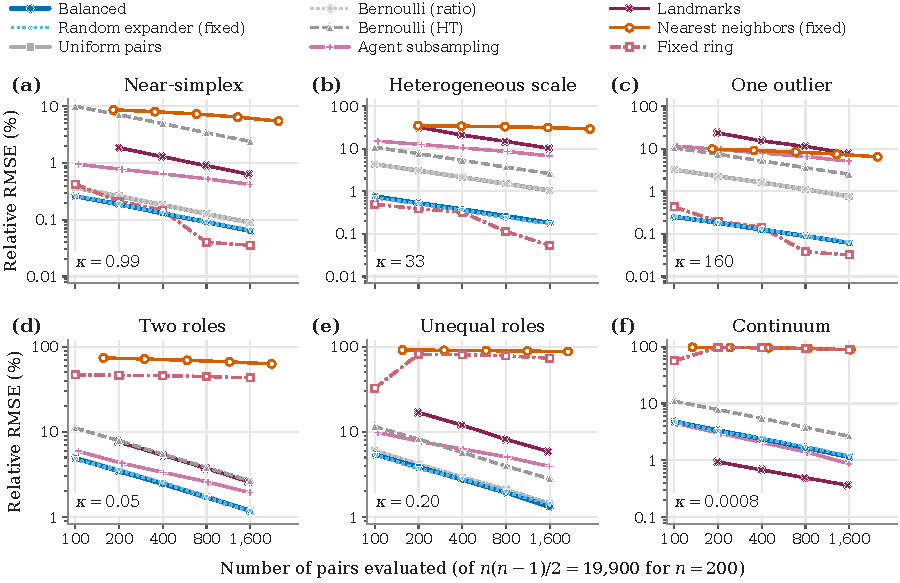
\includegraphics[width=\textwidth]{figures/fig_designs.pdf}
  \caption{\textbf{Error of every design across budgets.} Relative RMSE
  against the number of pairs evaluated for the six synthetic families of
  \Cref{tab:synthetic} ($n=200$; root mean square over three tables per
  family; \Cref{tab:e2} is the slice $m=2n$). Each design is plotted at the
  number of pairs it actually evaluates: symmetrized nearest-neighbor graphs
  use between $m$ and $2m$, and landmarks never fewer than $n-1=199$. The
  balanced (round-robin) design and a fixed random expander coincide in
  every family, as \Cref{thm:balanced} predicts for a regular graph drawn
  independently of the labels; where two designs coincide, the second
  (expander, Bernoulli (ratio)) is drawn dotted on top of the first. Uniform and Bernoulli (ratio) sampling
  overlap in every panel and coincide with the balanced design (drawn
  behind it) only when $\kappa\approx 0$. The nearest-neighbor
  graph, which is built from the table itself, is biased in every family,
  and its error barely decreases with $m$. The fixed ring is strongly biased only in
  the bottom row, where labels follow the generator's ordering; in the top
  row its expected squared error equals the balanced variance
  (\Cref{thm:balanced}), and the points are single realizations on three tables.}
  \label{fig:designs}
\end{figure}

\begin{figure}[!ht]
  \centering
  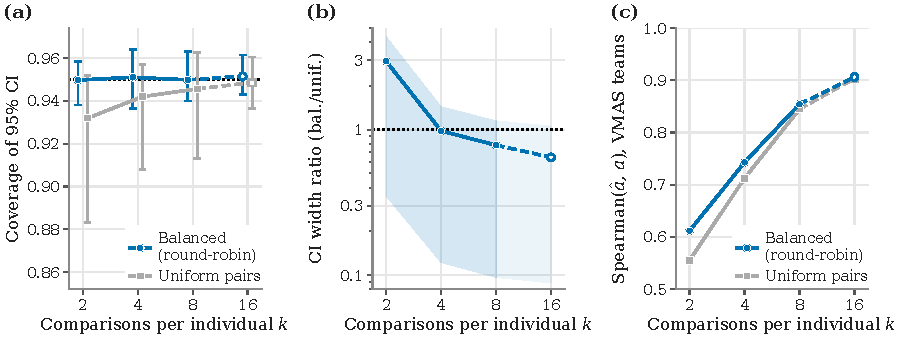
\includegraphics[width=\textwidth]{figures/fig_ci.pdf}
  \caption{\textbf{Error bars and distinctiveness from sparse balanced
  designs.} CI denotes a $95\%$ confidence interval. Results over $26$ tables: six synthetic families ($n=200$), the
  $128$-model population, and $19$ VMAS tables (four trained teams, $14$
  one-outlier and two-group variants, and one untrained $n=100$ team), with
  $2{,}000$ draws per table and
  $k$. At $k=16$ the design needs $n-1\ge16$ rounds, so only the $13$ tables
  with $n\ge32$ enter (dashed segments, open markers). (a) Coverage of nominal $95\%$
  intervals. Balanced (round-robin) intervals treat the $k$ round means as a
  simple random sample without replacement from the $n-1$ rounds, with a
  $t_{k-1}$ quantile and finite-population correction $1-k/(n-1)$. Markers
  show the mean over tables, bars the range over tables, and the dotted
  line the nominal level. Balanced intervals average $0.950$--$0.952$
  coverage at every $k$, whereas Wald intervals from uniform pairs
  undercover, down to $0.88$ on the synthetic one-outlier table at $k=2$.
  (b) Median width ratio, balanced/uniform (band: range over tables,
  lighter at $k=16$; dotted: equal width). The median ratio is $2.96$, $0.98$, $0.78$, and
  $0.65$ at $k=2$, $4$, $8$, and~$16$. At $k=2$ the median balanced interval is wider
  because the $t_1$ quantile ($12.7$) is $6.5$ times the normal one. For
  $k\ge4$ balanced intervals are up to $11\times$ narrower when distinctiveness dominates
  (one-outlier table) and at most $1.44\times$ wider when $\kappa\approx0$.
  (c) Rank correlation between estimated and true distinctiveness $a_i$ on
  the VMAS teams ($19$ tables; $6$ at $k=16$): four comparisons per individual
  already give a mean Spearman correlation of $0.74$ (first $300$ draws per
  table).}
  \label{fig:ci}
\end{figure}



% Moved from appendix_proofs.tex to the supplement (page budget).
% ------------------------------------------------------------
\section{Separable Dissimilarities Admit Exact Near-Linear-Time Evaluation}
\label{app:separable}

Balanced designs are needed only when $d$ admits no algebraic shortcut;
the following proposition gives two such shortcuts.

\begin{proposition}[Separable dissimilarities]
\label[proposition]{prop:separable}
Let $D$ be a dissimilarity table.
\begin{enumerate}
\item[(i)] Suppose $d_{ij}=f_i+f_j-2\langle\phi_i,\phi_j\rangle$ for scalars $f_i$
and vectors $\phi_i$ in a $q$-dimensional inner-product space. Then
\[
\SND(D)=\frac1N\Big[(n-1)\sum_i f_i+\sum_i\norm{\phi_i}^2-\Big\|\sum_i\phi_i\Big\|^2\Big],
\]
which is computable exactly in $O(nq)$ operations. Examples include squared
Euclidean distance ($f_i=\norm{x_i}^2$, $\phi_i=x_i$), giving the variance
identity ${\SND=2\sum_i\norm{x_i-\bar x}^2/(n-1)}$. Further
examples are squared $W_2$ between Gaussians $\mathcal N(m_i,\Sigma_i)$ with
pairwise commuting (for example diagonal) covariances, with
$f_i=\norm{m_i}^2+\operatorname{tr}\Sigma_i$ and $\phi_i=(m_i,\Sigma_i^{1/2})$; squared
Hellinger distance $\tfrac12\lVert\sqrt{\pi_i}-\sqrt{\pi_j}\rVert^2$ between
distributions $\pi_i$ on $q$ outcomes, with $\phi_i=\sqrt{\pi_i}/\sqrt2$ and $f_i=\frac12$;
cosine dissimilarity $1-\cos(x_i,x_j)$, with $\phi_i=x_i/(\sqrt2\,\norm{x_i})$ and
$f_i=\frac12$; LPIPS-type squared feature distances; and $0$--$1$
disagreement between categorical outputs ($\phi_i=e_{y_i}/\sqrt2$, $f_i=\frac12$).
\item[(ii)] Suppose $d_{ij}=\sum_{c=1}^q\abs{x_{ic}-x_{jc}}$, an $\ell_1$
dissimilarity. This includes total variation between categorical action
distributions, averaged over observations. Then
\[
\sum_{i<j}d_{ij}=\sum_{c=1}^q\sum_{t=1}^n(2t-n-1)\,x_{(t)c},
\]
where $x_{(1)c}\le\dots\le x_{(n)c}$ are the sorted values of coordinate $c$. This is
computable exactly in $O(q\,n\log n)$ operations.
\end{enumerate}
\end{proposition}

\begin{proof}
\emph{(i)} $\sum_{i<j}(f_i+f_j)=(n-1)\sum_if_i$, and
$\sum_{i<j}\langle\phi_i,\phi_j\rangle=\frac12\big(\norm{\sum_i\phi_i}^2-\sum_i\norm{\phi_i}^2\big)$.
For squared Euclidean distance, $(n-1)\sum_i\norm{x_i}^2+\sum_i\norm{x_i}^2-\norm{\sum_i x_i}^2=n\sum_i\norm{x_i-\bar x}^2$,
and $N=n(n-1)/2$. \emph{(ii)} For sorted values,
$\sum_{s<t}(x_{(t)}-x_{(s)})=\sum_t x_{(t)}\big[(t-1)-(n-t)\big]$, and the
coordinates add.
\end{proof}

\begin{remark}[Non-separable dissimilarities and metric scope]
Many dissimilarities are of neither form (i) nor form (ii). Examples are unsquared
Euclidean distance in dimension $q\ge2$, Hellinger distance, $W_2$ between
Gaussians (hence SND as defined by \citealt{bettini2025snd}), Jensen--Shannon
distance, edit and optimal-transport distances between trajectories, and
rollout- or judge-based comparisons. Univariate $W_1$, by contrast, is the
$\ell_1$ distance between cumulative distribution functions, so for
distributions on a common finite grid it is covered by (ii). Distances with explicit Euclidean
embeddings, $d_{ij}=\norm{x_i-x_j}_2$, admit a further, randomized shortcut. Since
$\E_g\abs{\langle v,g\rangle}=\sqrt{2/\pi}\,\norm v$ for $g\sim\mathcal N(0,I_q)$, random
one-dimensional projections combined with (ii) give unbiased estimates of $\mu$
that touch every individual. This is the projection-based approach of
\citet{barhum2007approximating}, and its accuracy is set by the number of
projections. Balanced designs need no embedding, only black-box access to $d$,
and are therefore the tool of choice when no embedding is available.
Theorem~\ref{thm:balanced} covers every dissimilarity table, whether or not it is
a metric. Theorem~\ref{thm:metric} applies only to pseudometric tables. These
include exactly computed Euclidean, Hellinger, Jensen--Shannon, edit and
$W_p$ optimal-transport distances (including $W_2$); they exclude comparisons that can violate the
triangle inequality: Kullback--Leibler divergences, cross-play return gaps, entropic (Sinkhorn)
transport costs, dynamic-time-warping alignments, judge scores, and Monte Carlo
estimates of distances that use different samples for different pairs (averages over one shared sample, such as the common observation pool of SND, remain pseudometrics).
\end{remark}



% Proofs and remarks moved from appendix_proofs.tex to the supplement (page budget).
\section{Additional Proofs and Remarks}
\label{app:supp-proofs}

\subsection{Classical counterparts of the anatomy}

\begin{remark}[Classical counterparts]
In Theorem~\ref{thm:anatomy}, parts (i) and (ii) identify the anatomy with the
two-way analysis of variance (ANOVA) of a symmetric layout.
This decomposition is exactly Griffing's Method~4 diallel analysis, which splits crosses into
general and specific combining ability \citep{griffing1956concept}. It is also
the finite-population (without-replacement) Hoeffding decomposition of the pair
average \citep{nandi1963properties,bloznelis2001orthogonal}, and the symmetric social relations model \citep{kenny1984social}. The
classical i.i.d.\ Hoeffding projection \citep{hoeffding1948class} differs by the
factor $(n-2)/n$ on the main effects. The double centering of classical scaling
\citep{torgerson1952multidimensional,gower1966some} removes the same main effects,
but it acts on the $n\times n$ matrix including its diagonal. Our residual is
centered on the $N$ off-diagonal pairs, and this centering is what makes
\Cref{prop:error-identity,thm:balanced} exact. It is the U-centering of
\citet{szekely2014partial}, which \citet{zhang2026ucentering} characterizes as
the least-squares residual after fitting additive endpoint effects.
\end{remark}

\subsection{Relation to incomplete U-statistics}

\begin{remark}[Relation to incomplete U-statistics]
\label[remark]{rem:classical}
For i.i.d.\ observations, the variance of an incomplete U-statistic depends
on a fixed design only through its degree sequence, and equireplicate
designs minimize it
\citep{blom1976some,brown1978reduced,lee1982incomplete,lee1990ustatistics}.
As in that setting, where a regular design has the same H\'ajek projection
as the complete statistic, regularity removes the main effects from the
error, here in every realization, and \Cref{thm:balanced}(iii) is the
permutation variance of a quadratic-assignment statistic
\citep{daniels1944relation,mantel1967detection,hubert1987assignment},
expressed through the anatomy. Within the variance formula itself, only the finite-population correction
differs: residuals of overlapping pairs have covariance
$-\sigmaint/(n-2)$ (\Cref{lem:corr}), so for
${\kappa<2(n-1)/\bigl(n(n-3)\bigr)}$ irregular designs such as landmarks have
smaller variance than regular ones (\Cref{thm:general-design}), while
uniform pair sampling gains at most the factor
$1+2(n-1)/\bigl(n(n-3)\bigr)$ (\Cref{cor:efficiency}). Over an i.i.d.\
superpopulation, equireplicate designs are again optimal
(\Cref{sec:discussion}).
\end{remark}

\subsection{Energy per dimension}

\begin{remark}[Energy per dimension]
\label[remark]{rem:dof}
The two variances have the same form,
\[
\Var(T)=\frac{N-m}{m}\cdot\frac{\sigmaint}{n(n-3)/2},
\qquad
\Var(T_U)=\frac{N-m}{m}\cdot\frac{\sigmatot}{N-1}.
\]
Uniform sampling is exposed to the total energy, spread over all $N-1$
non-constant directions of $\R^{\Pairs}$; a balanced design is exposed only
to the relational energy, spread over the $n(n-3)/2$ dimensions of the
relational subspace (\Cref{thm:anatomy}(iii)). The threshold of
\Cref{cor:efficiency} is the ratio $(n-1)/\bigl(n(n-3)/2\bigr)$ of the
dimensions of the distinctiveness and relational subspaces, so balance pays
off exactly when distinctiveness carries more energy per dimension than
relational structure does.
\end{remark}

\subsection{Why Chebyshev and a median}

\begin{remark}[Why Chebyshev and a median]
\label[remark]{rem:why-median}
A single balanced design also concentrates exponentially: once the labels are
randomized, $T$ is a function of a uniform permutation, so bounded-difference
inequalities for permutations apply \citep{mcdiarmid1989method}. These bounds
depend on the range of the table. Swapping two labels changes up to $2k$
compared pairs, hence $T$ by up to $4d_{\max}/n$, where
$d_{\max}=\max_{i<j}d_{ij}$, so the resulting exponent is of order
$n\varepsilon^2\mu^2/d_{\max}^2$ and does not improve with $k$. Over
pseudometrics the ratio $d_{\max}/\mu$ can grow linearly in $n$: one
individual at unit distance from $n-1$ coincident others gives $\mu=2/n$ and
$d_{\max}/\mu=n/2$, and the bound is then vacuous. Chebyshev's inequality
needs only $\Var(T)/\mu^2\le v_{n,k}\le 2/(nk)$, which \Cref{thm:metric}
establishes for every pseudometric without reference to $d_{\max}$. The
median of $L=\lceil 8\ln(1/\eta)\rceil$ independent designs
(\Cref{lem:median}) then restores the $\log(1/\eta)$ dependence. The
guarantee is therefore scale-free: it holds uniformly over pseudometric
tables, including tables with arbitrary outliers. When $d_{\max}/\mu$ is
known to be bounded, a single design with a tail bound is a valid
alternative.
\end{remark}

\subsection{Higher moments of balanced designs}

\begin{remark}[Higher moments depend on the design]
Only the first two moments of the error $T-\mu$ of a balanced design (Theorem~\ref{thm:balanced}) are free of its base graph $H$. Third and higher moments
involve counts of small subgraphs of $H$, such as triangles and paths. For example,
at $n=6$ and $k=2$ the hexagon and two disjoint triangles give identical means and
variances but, in general, different third moments. Tail bounds sharper than Chebyshev's
therefore depend on the chosen $H$, while all of our guarantees use only the
variance.
\end{remark}

\subsection{Proof of Proposition~\ref{prop:lower}}
\label{app:lower}

\begin{proof}
Both constructions are standard in the sublinear-algorithms literature
\citep{barhum2007approximating,goldreich2008approximating}. We include them so
the constants are explicit.

\emph{(i)} Let $D^{(0)}$ have all off-diagonal entries equal to $1$ (so $\mu=1$).
For $u\in[n]$, let $D^{(u)}$ agree with $D^{(0)}$ except $d_{uj}=1+n$ for $j\neq u$.
Then $\mu(D^{(u)})=1+n(n-1)/N=3$. Both tables are pseudometrics: the only
nontrivial checks are $1+n\le(1+n)+1$ and $1\le2(1+n)$. The intervals
$(3^{-1/2},3^{1/2})$ and $(3^{1/2},3^{3/2})$ are disjoint, so a procedure that
succeeds on $D^{(0)}$ and on $D^{(u)}$ must distinguish them. Run the procedure with
the same internal randomness on $D^{(0)}$ and on $D^{(u)}$. Both runs see identical
answers until a pair containing $u$ is queried. Let $V_0$ be the set of individuals
touched by the $q<n/8$ queries of the run on $D^{(0)}$, so $\abs{V_0}\le2q$. If $u\notin V_0$,
the two runs coincide and produce the same output, so at least one of them fails.
Draw $u$ uniformly and independently of the internal randomness. Then
$\Prob(u\in V_0)\le 2q/n<1/4$, and
$\Prob(\text{fail on }D^{(0)})+\E_u\Prob(\text{fail on }D^{(u)})\ge\Prob(u\notin V_0)>3/4$.
Hence some table in the family has failure probability greater than $3/8$.

\emph{(ii)} Let $P_\pm$ be the laws of random symmetric tables whose entries $d_{ij}$, $i<j$, are
independently $2$ with probability $\tfrac12\pm\varepsilon$, and $1$ otherwise.
Every such table is a pseudometric, since all entries lie in $[1,2]$. Under
$P_\pm$, $\mu=1+B/N$ with $B\sim\mathrm{Bin}(N,\tfrac12\pm\varepsilon)$. By
Chebyshev, $P_\pm\big(\abs{\mu-(\tfrac32\pm\varepsilon)}>\varepsilon/8\big)\le
16/(N\varepsilon^2)\le1/256$ when $N\ge4096\,\varepsilon^{-2}$. On
the complementary events, a $(1\pm\varepsilon/2)$-approximation $\widehat\mu$
satisfies $\widehat\mu>\tfrac32$ under $P_+$ and $\widehat\mu<\tfrac32$ under
$P_-$, since $\varepsilon\le1/8$. So a procedure with worst-case success
probability $2/3$ yields a test between $P_+$ and $P_-$ with average success at
least $2/3-1/256>0.66$. Hence the total variation between the transcript laws
satisfies $\mathrm{TV}\ge0.32$. Repeated queries reveal nothing new, so assume
$q$ distinct queries. Each reveals an independent
$\mathrm{Bernoulli}(\tfrac12\pm\varepsilon)$ entry, even under adaptivity. By the
chain rule and the $\chi^2$ bound on the Kullback--Leibler (KL) divergence,
$\mathrm{KL}\le q\,(2\varepsilon)^2/(\tfrac14-\varepsilon^2)\le 18\,q\,\varepsilon^2$.
Pinsker's inequality gives $0.32\le\mathrm{TV}\le\sqrt{9q\varepsilon^2}$, so
$q\ge0.011\,\varepsilon^{-2}$.

\emph{Combining (i) and (ii).} A $(1\pm\varepsilon/2)$-approximation with
$\varepsilon\le1/8$ lies in $(3^{-1/2},3^{1/2})\mu$. A procedure that succeeds with
probability $2/3>5/8$ on every pseudometric table therefore needs at least $n/8$
evaluations by (i) and, when $N\ge4096\,\varepsilon^{-2}$, at least $c\,\varepsilon^{-2}$ by (ii). It thus needs at
least $\tfrac12(n/8+c\,\varepsilon^{-2})$.

\emph{(iii)} Under uniform sampling with replacement, each draw contains $u$ with
probability $(n-1)/N=2/n$. In that case it returns $1+n$, and otherwise $1$. Hence
a single draw $d$ has $\Var(d)={n^2\cdot\frac2n\bigl(1-\frac2n\bigr)}=2(n-2)$. Since
$\mu=3$ and the $m$ draws are independent, $\Var(T_U')/\mu^2=2(n-2)/(9m)$. Finally, $d^{(u)}_{ij}=3+a_i+a_j$ with $a_u=n-1$
and $a_l=-1$ for $l\neq u$, so $\sum_ia_i=0$. Uniqueness in
Theorem~\ref{thm:anatomy}(i) gives level $3$, distinctiveness $a$ and $R=0$.
Theorem~\ref{thm:balanced}(i) then shows that every balanced design is exact.
\end{proof}

% ------------------------------------------------------------
\subsection{Proof of Proposition~\ref{prop:sparse-anatomy}}
\label{app:supp-sparse-dico}

\begin{proof}
Write $u=\sigma^{-1}(i)$ for the vertex of $H$ that receives individual $i$.
Since $\sigma$ is uniform, $u$ is uniform on $[n]$. Conditional on $u$, the
restriction of $\sigma$ to $[n]\setminus\{u\}$ is a uniform bijection onto
$[n]\setminus\{i\}$. The partners of $i$ in $G$ are the images of the $k$
neighbors of $u$ in $H$, so they form a uniformly random $k$-subset of
$[n]\setminus\{i\}$, whatever $u$ is. Hence $\widehat m_i$ is the mean of a simple
random sample of size $k$, drawn without replacement from the $n-1$ values
$\{d_{ij}\}_{j\ne i}$. These values have mean $S_i/(n-1)$ and population variance
$s_i^2$ (divisor $n-1$). The standard finite-population formula
\citep{cochran1977sampling} gives $\E[\widehat m_i]=S_i/(n-1)$ and the stated
$\Var(\widehat m_i)$. By Theorem~\ref{thm:balanced}, $\E[T]=\mu$, so
\[
\E[\widehat a_i]=\frac{n-1}{n-2}\Big(\frac{S_i}{n-1}-\mu\Big)=\frac{S_i-(n-1)\mu}{n-2}=a_i .
\]
Finally, $\widehat a_i-a_i=\frac{n-1}{n-2}\big[(\widehat m_i-\E[\widehat m_i])-(T-\mu)\big]$
and $(x-y)^2\le2x^2+2y^2$ give the stated bound on $\Var(\widehat a_i)$.
\end{proof}

% ------------------------------------------------------------
\subsection{Proof of Proposition~\ref{prop:dico}}\label{app:supp-dico}

\begin{proof}
Homogeneity gives $\SND(c\,h)=c\,\SND(h)$, so
$\SND_{\mathrm{real}}=\SNDdes\,\SND(h)/\widehat{\SND}=\SNDdes/(1+e)$.

\emph{(i)} If $\abs e\le\varepsilon<1$, then
$\lvert 1/(1+e)-1\rvert=\lvert e\rvert/(1+e)\le\varepsilon/(1-\varepsilon)$.

\emph{(ii)} On the event $\{T=0\}$ we have $e=-1$. This event lies inside
$\{\abs e>\varepsilon\}$ and inside $\{\abs e>1/2\}$, so the convention
$1/\SND_{\mathrm{real}}:=0$ there affects none of the bounds below.
Theorem~\ref{thm:balanced}(ii) gives $\E[e]=0$, so
$\E[1/\SND_{\mathrm{real}}]=\E[1+e]/\SNDdes=1/\SNDdes$. By (i), the event
$\{\abs{\SND_{\mathrm{real}}/\SNDdes-1}>\varepsilon/(1-\varepsilon)\}$ is contained
in $\{\abs e>\varepsilon\}$. Chebyshev's inequality and \mbox{Theorem}~\ref{thm:metric}
bound the probability of the latter by $\E[e^2]/\varepsilon^2\le v_{n,k}/\varepsilon^2$.
For the bias, write ${1/(1+e)-1=-e+e^2/(1+e)}$. Since $\E[e]=0$,
$-\E[e\,\one\{\abs e\le\frac12\}]=\E[e\,\one\{\abs e>\frac12\}]$, whose absolute value
is at most $2\E[e^2]$. On $\{\abs e\le\frac12\}$ we have $e^2/(1+e)\le2e^2$.
Summing the two bounds gives $4\E[e^2]$. Markov's inequality gives
$\Prob(\abs e>\frac12)\le4\E[e^2]$.
\end{proof}



\vskip 0.2in
\setlength{\bibsep}{2pt plus 0.3ex}
\bibliography{refs}
\label{supp:last}

\end{document}
